Как говорилось ранее, приложение будет производить много работы с файлами, расположенными на диске. По этой причине удобно сформировать определённую иерархию папок, чтобы размещать в них файлы, а также "--- реализовать методы для удобного доступа к этим файлам.

Рассмотрим подробно иерархию папок, которая используется в нашем приложении. Корневая папка \texttt{file\_system} содержит четыре подпапки:

\begin{itemize}
\item \texttt{problems} "--- содержит пронумерованные папки со всеми файлами, относящимися к определённой задаче;
\item \texttt{submissions} "--- содержит пронумерованные папки с исходным кодом и скомпилированными файлами отправленных посылок;
\item \texttt{temp} "--- содержит временные файлы, периодически создаваемые и удаляемые приложением;
\item \texttt{config} "--- содержит конфигурационные файлы (необходимые, например, для корректной компиляции программ и их выполнения в модуле тестирования).
\end{itemize}

Каждая папка с посылкой содержит внутри себя XML-дескриптор, описывающий параметры посылки, и две папки "--- \texttt{src} c исходным кодом и \texttt{bin} со скомпилированным файлом. Сразу заметим, что способ хранения этих файлов аналогичен для авторских решений и средств разработки задач, что отражается на способе доступа к ним из программы.

Каждая папка с задачей так же содержит XML-дескриптор с параметрами задачи, условие (файл \texttt{statement.pdf}) и ещё несколько папок:

\begin{itemize}
\item \texttt{tests} "--- содержит по одной папке для каждой группы тестов, каждая из которых, в свою очередь, содержит XML-дескриптор группы тестов и пронумерованные папки с тестами (каждый тест представлен двумя файлами: \texttt{input.txt} и \texttt{output.txt});
\item \texttt{checker} "--- содержит две папки \texttt{src} и \texttt{bin} с файлами единственного чекера, прикреплённого к задаче;
\item \texttt{generators} "--- содержит набор пронумерованных папок с файлами генераторов (разложенных так же по папкам \texttt{src} и \texttt{bin});
\item \texttt{validators} "--- с пронумерованными папками для файлов валидаторов (разложенных по папкам \texttt{src} и \texttt{bin});
\item \texttt{author\_decisions} "--- с пронумерованными папками для файлов авторских решений (разложенных по папкам \texttt{src} и \texttt{bin}) и XML-дескриптором авторского решения.
\end{itemize}

Классы модуля для работы с файловой системы также разложены по пакетам. Отдельные пакеты отведены для классов, ответственных за иерархию папок, за обращение с XML-дескрипторами и за логирование. На рис.~\ref{package_diagram_file_system} отражена структура данного модуля.

\begin{figure}[h]
\center{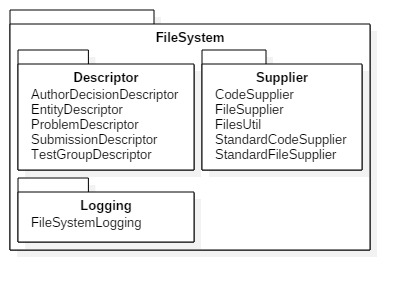
\includegraphics[scale=0.8]{package_diagram_file_system}}
\caption{Модуль для работы с файловой системой}
\label{package_diagram_file_system}
\end{figure}

Интерфейс \texttt{File\-Supplier} предоставляет все методы, необходимые для работы с перечисленными файлами и папками, в том числе методы для их добавления, удаления и доступа к ним. Интерфейс устроен таким образом, что каждая задача, посылка, тест и любая другая сущность однозначно идентифицируется в своём контексте некоторым числовым идентификатором, соответствующим имени папки, в которой она расположена. Предоставляемая реализация интерфейса "--- класс \texttt{Standard\-File\-Supplier} "--- для выполнения однотипных операций с файлами использует множество статических методов вспомогательного класса \texttt{Files\-Util}. Также в момент инициализации класс \texttt{Standard\-File\-Supplier} принимает путь, по которому следует искать и располагать всю используемую иерархию папок.

Как уже говорилось выше, поскольку способ хранения исходного кода и скомпилированных программ одинаков для разных сущностей, для доступа к ним удобно добавить свой интерфейс. В роли такого интерфейса выступает \texttt{Code\-Supplier}, который можно получить, вызвав некоторые из методов \texttt{File\-Supplier}. Данный интерфейс не только даёт доступ к соответствующим файлам и папкам, но также даёт возможность положить в папку новый файл с исходный кодом. Используемая реализация этого интерфейса "--- класс \texttt{Standard\-Code\-Supplier}.

Некоторым из используемых сущностей также соответствуют некоторые свойства, которые хранятся в виде XML-файлов. Главный класс, реализующий взаимодействие с такими XML-дескрипторами "--- \texttt{Entity\-Descriptor}. Он хранит в себе объект типа \texttt{Map}, в котором ставятся в соответствие имена свойств и их значения. Помимо методов доступа и установки этих значений класс \texttt{Entity\-Descriptor} предоставляет также методы \texttt{load()} и \texttt{persist()} для автоматической загрузки и сохранения свойств из соответствующего файла.

Каждой из сущностей, имеющих специальные свойства, соответствует некоторый класс, наследующий от \texttt{Entity\-Descriptor}. Всего таких классов четыре:

\begin{itemize}
\item \texttt{Problem\-Descriptor} "--- содержит название задачи, ограничения по времени и по памяти и используемый в задаче тип проверки корректности ответа;
\item \texttt{Submission\-Descriptor} "--- содержит идентификатор соответствующих задачи, системы оценивания и компилятора, а также вердикт по посылке, присуждённые очки, номер первого неудачного теста и использованные решением время и память;
\item \texttt{Author\-Decision\-Descriptor} "--- содержит название авторского решения и идентификатор компилятора;
\item \texttt{Test\-Group\-Descriptor} "--- содержит количество очков, присуждаемых за один тест из данной группы тестов.
\end{itemize}